\documentclass[a4paper, 12pt]{article}
\usepackage{cmap}           % Пакет для поиска в полученной пдфке
\usepackage[utf8]{inputenc} % Ззамена кодировки файла на utf8
\usepackage[T2A]{fontenc}   % Подключение кодировки шрифтов
\usepackage[russian]{babel} % Использование русского языка 
\usepackage[left=2cm, right=2cm, top=1cm, bottom=2cm]{geometry} % Изменение размеров полей
\usepackage{indentfirst}    % Красная строка в начале текста
\usepackage{amsmath, amsfonts, amsthm, mathtools, amssymb, icomma, units, yfonts}
\usepackage{amsthm} % Пакет для нормального оформления теорем
\usepackage{graphicx}
\usepackage{tikz}
\usepackage{esvect}
\usetikzlibrary{calc,matrix}

%Теоремы
\newtheorem*{standartbase}{Теорема о стандартном базисе}
\newtheorem*{fulllemma}{Лемма}
\newtheorem*{sl1}{Следствие 1}
\newtheorem*{sl2}{Следствие 2}
\newtheorem*{monotonousbase}{Теорема о монотонном базисе}
\newtheorem*{scheme}{Утверждение 1}
\newtheorem*{n2}{Утверждение 2}

\renewcommand{\qedsymbol}{\textbf{Q.E.D.}}

\begin{document}
\title{Дискретная математика. Модуль 3. Лекция 1}
\author{Клуб альтруистичных и настойчивых}
\date{11 января 2016}

\maketitle
\section*{Схемы. Булевы схемы}
\textsc{Важное примечание:} В данной лекции все рассмотренные функции являются \textit{всюду определенными}.

\textit{Схема} --- это функция, заданная последовательность присваиваний.

Также в профессиональной среде схемы принято называть SLP (\textit{straight line programmes}). 

Рассмотрим такую функцию $f$, определенную для булевых значений (\textit{булеву функцию}): $f:\{0, 1\}^n \rightarrow \{0, 1\}$.

\textit{Базисом} B булевой функции будем называть некий набор $B:\{f_1, f_2, \ldots , f_n\}$, где $f_1 \ldots f_n$ - булевы функции.

\textit{Булева схема} в базисе B  --- последовательность функций $x_1, x_2, x_3... x_n, x_{n+1} := S_1, x_i := S_{L-n}$, которая вычисляет $x_L(x_1, \ldots ,x_n)$. 

\[S_j = g(S_{i_1},  ... , s_{i_r}), g \in B, i_\mathalpha < j\]

\textit{Стандартный базис} есть базис, состоящий из операций отрицания, конъюнкции и дизъюнкции: $\{\lnot, \vee, \wedge\}$

\textsc{Пример 1}

Cтандартный базис.
$x_1, \ldots x_n, s_1 := \lnot x_1, s_2 = \lnot x_2, s_3 := x_1 \wedge s_2, s_4 = x_2 \wedge s_1; s_5 = s_3 \vee s_4$

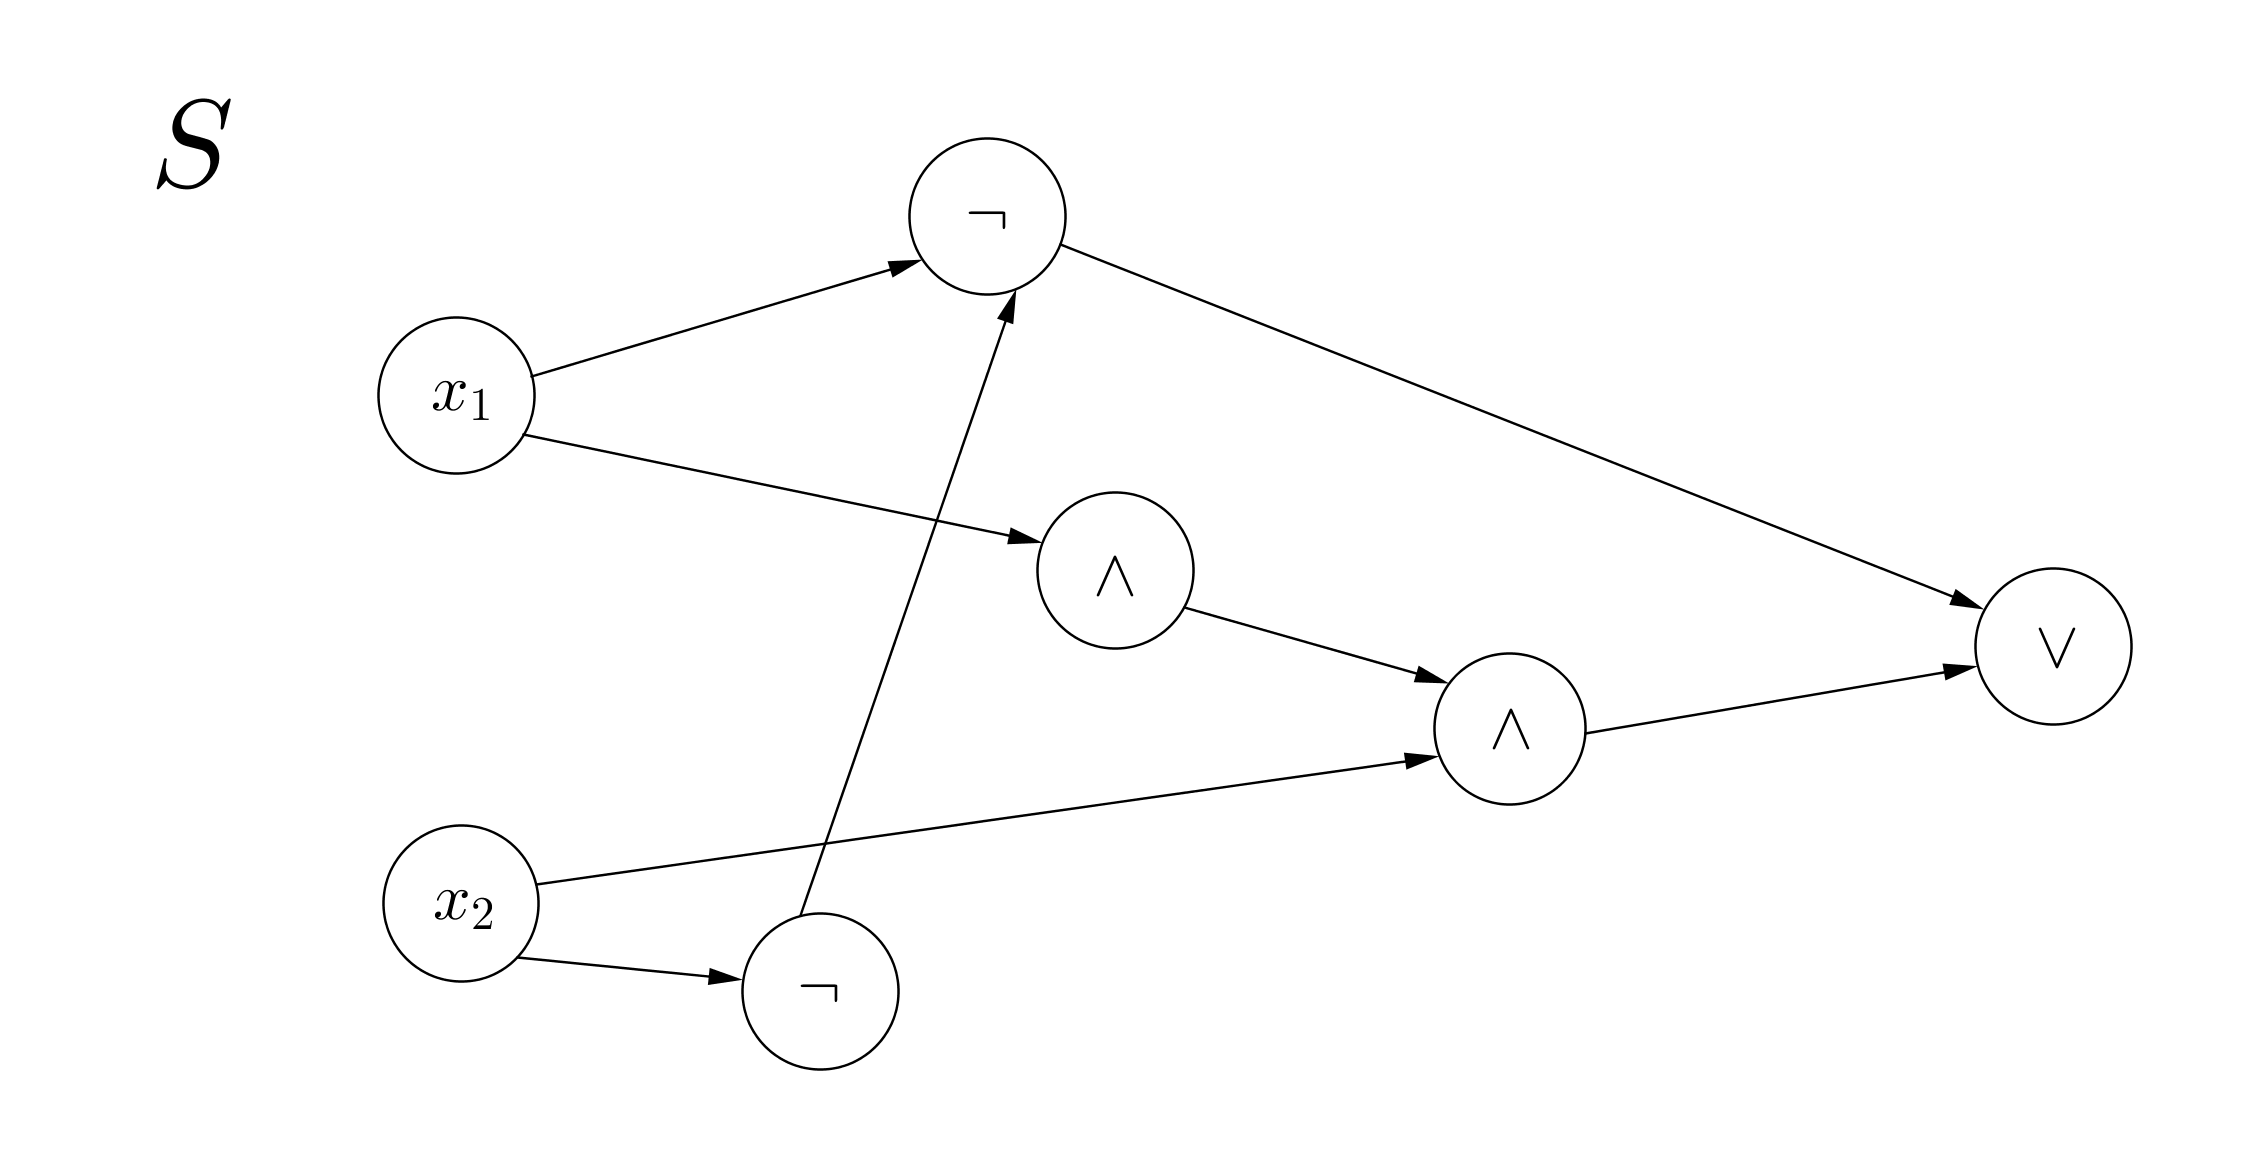
\includegraphics[height=7cm]{Images/1.png}
 
 Если $x_2 = 0$, то $s_5 = x_1$
  
 Если $x_2 = 1$, то $s_5 = \lnot x_1$
 
 Результатом является сложение по модулю 2 (1, если значения $x_1$ и $x_2$ разные) - $\oplus$.
 
 \textsc{Пример 2}
 
 Составим схему которая является xor нескольких переменных. Индуктивное доказательство существования такой функции:
  
$ x_1 \oplus x_2 \oplus \ldots \oplus x_{n-1} \oplus x_n = (x_1 \oplus x_2 \oplus \ldots \oplus x_{n-1}) \oplus x_n$
 
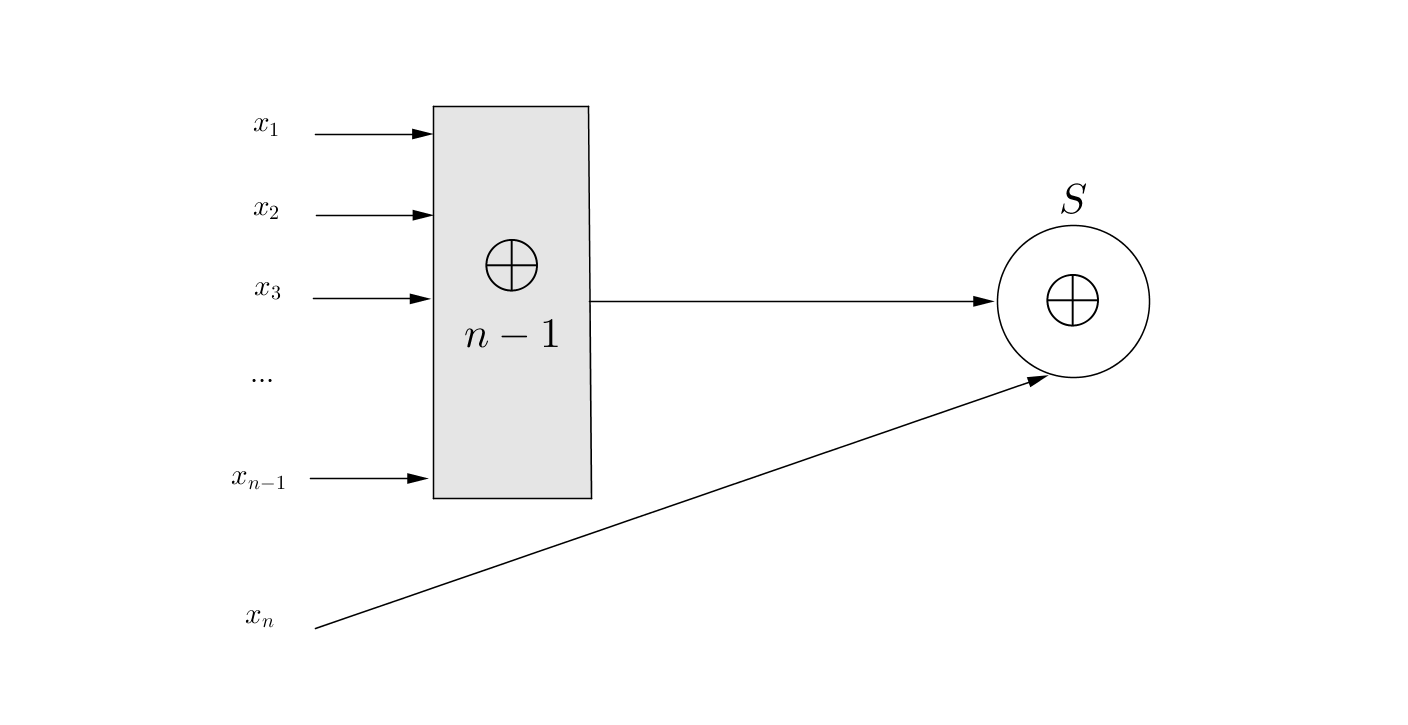
\includegraphics[height=7cm]{Images/2.png}
 
 \textsc{Пример 3}
 
 Дизъюнкция n переменных --- аналогично, по индукции. Такие рассуждения можно построить и для конъюнкции.
 
 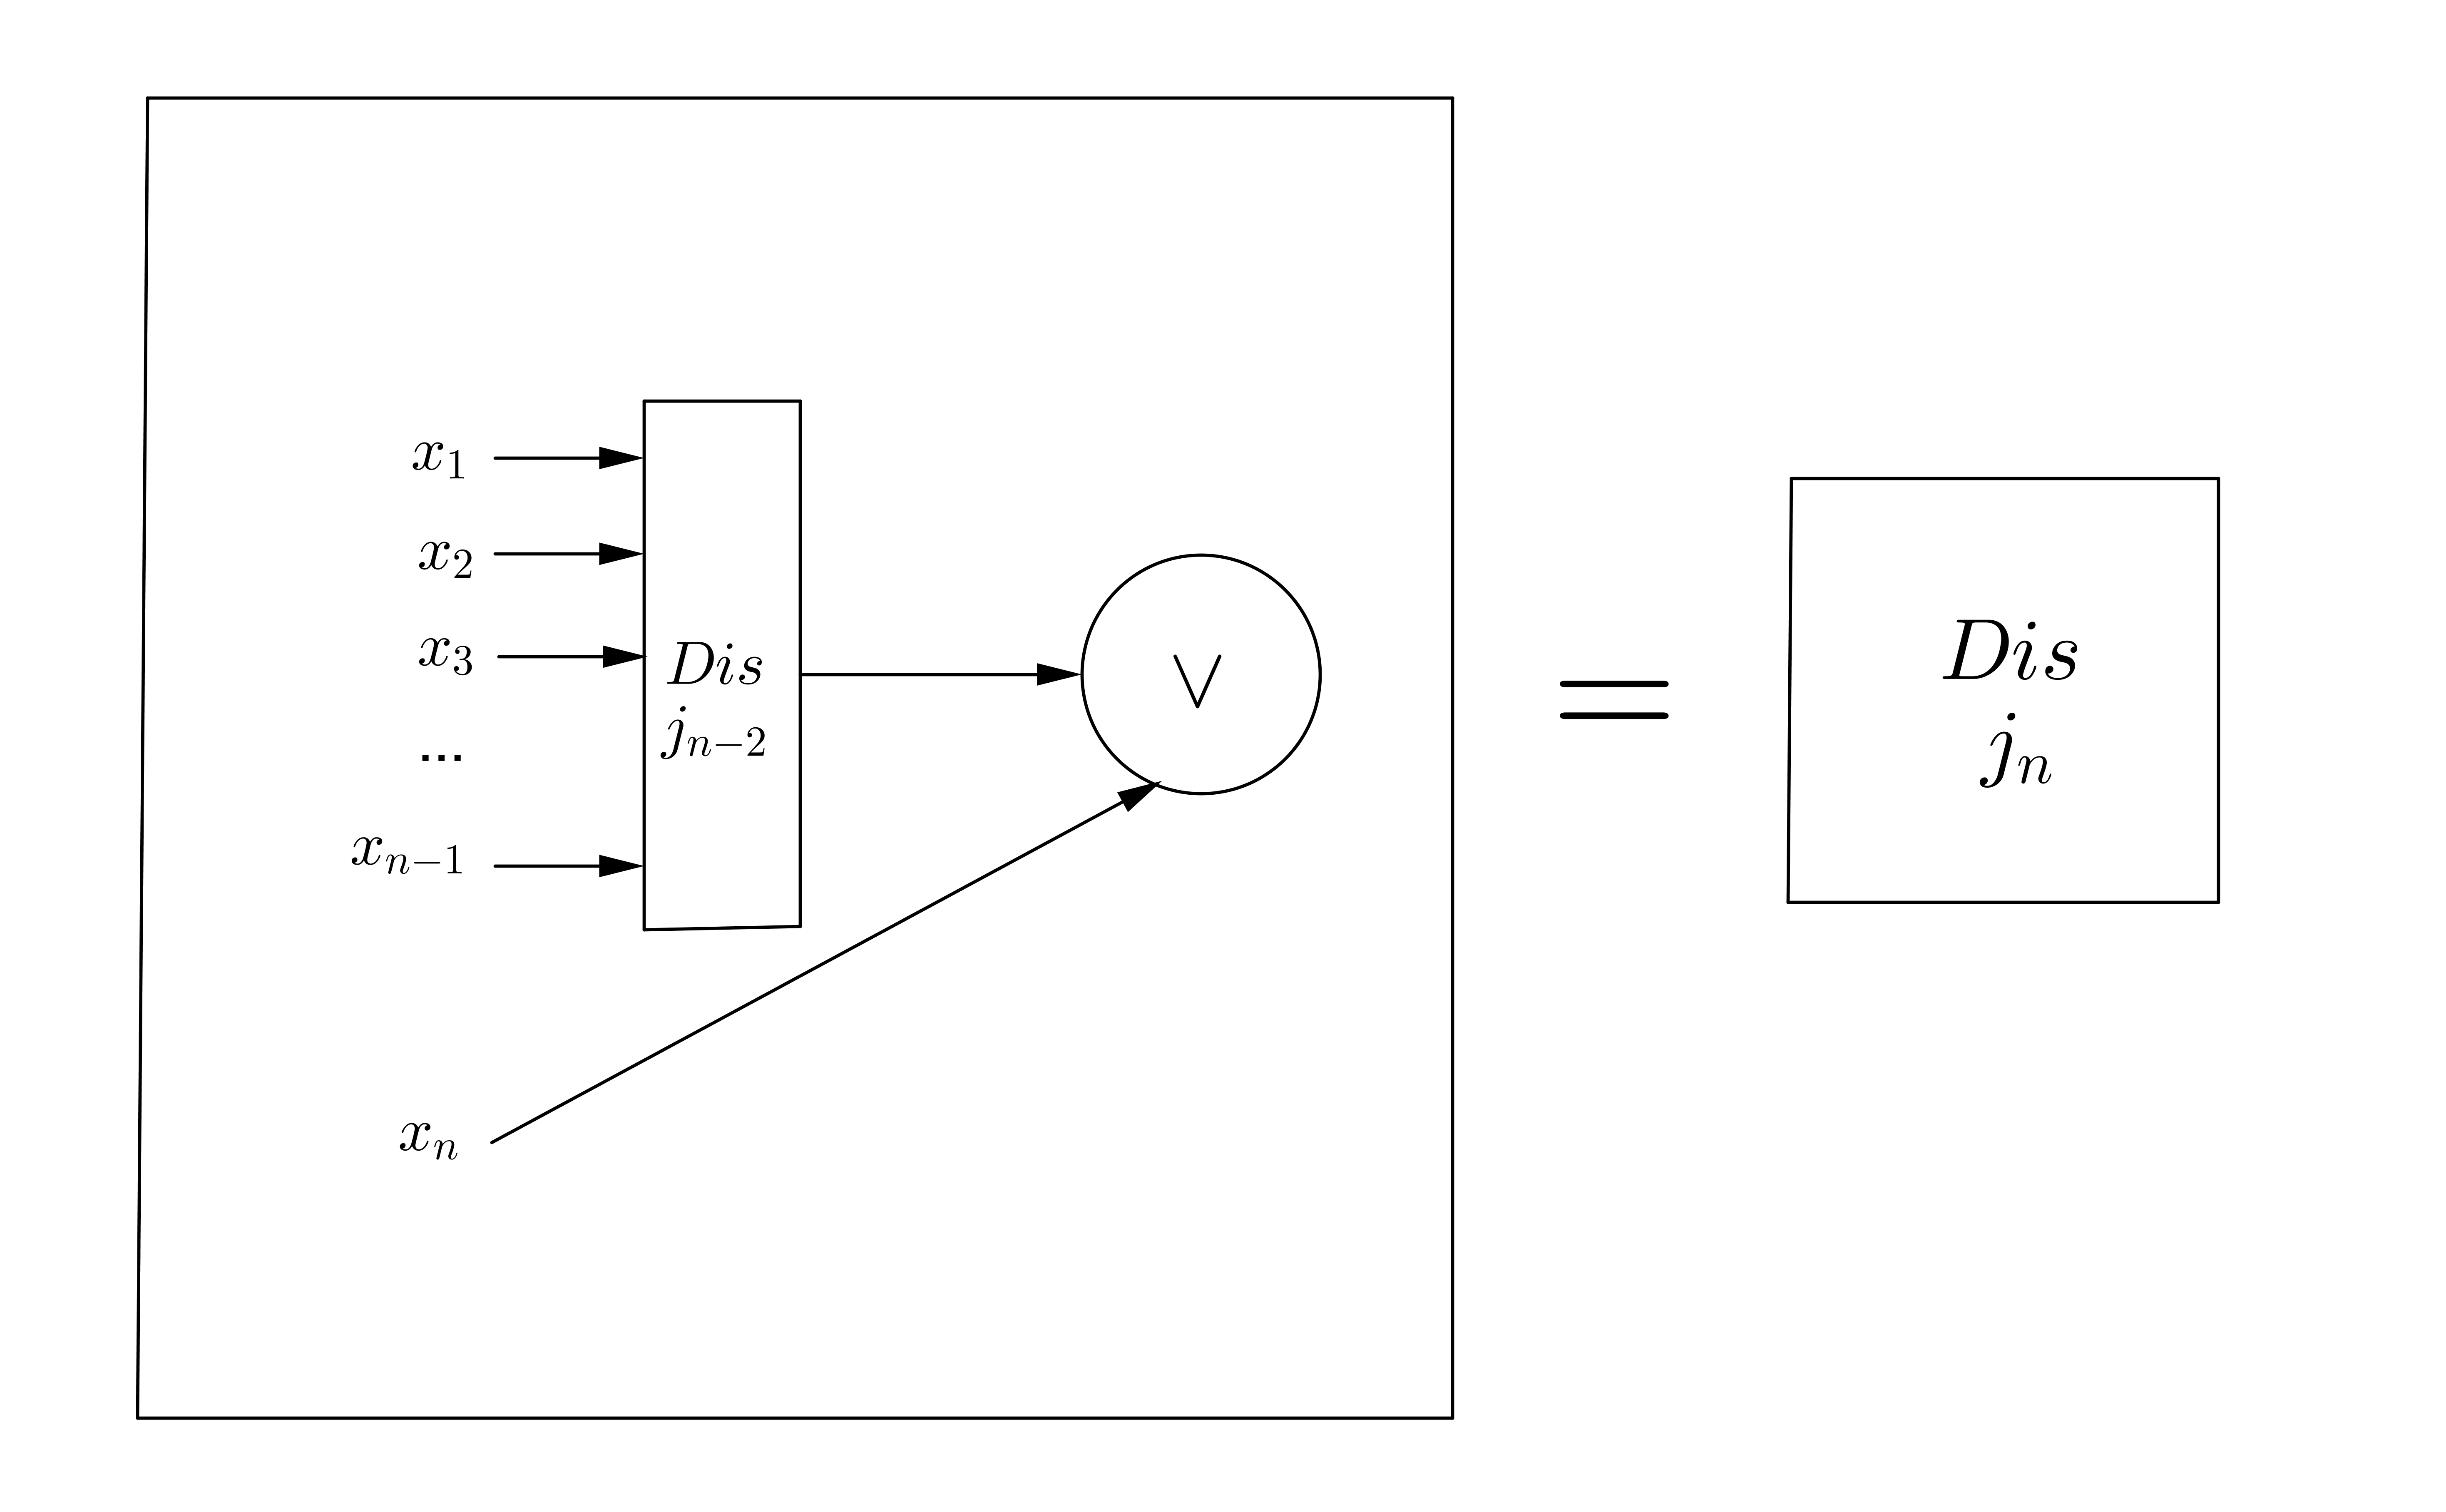
\includegraphics[height=7cm]{Images/3.png}
 
 \section*{Анализ схем}
 
 \textit{Анализ базисов: } все ли функции можно выразить через схему в данном базисе?
 
 \textit{Полный базис: } Базис B - \textit{полный}, если любую булеву функцию можно вычислить схемой в базисе B.
 
 \begin{standartbase}
 Стандартный базис --- полный.
 \end{standartbase}
 \begin{proof}
Вспомним, что ДНФ - это дизъюнкция конъюнктов литералов. Построим схему ДНФ.

$x_1, \ldots ,x_n, \lnot x_1, \ldots ,\lnot x_n, c_1, \ldots ,c_n, D$, где $c_j$ --- конъюнкция литералов, D --- дизъюнкция. Данный порядок действий соответствует определению ДНФ, следовательно ДНФ представима в виде схемы и любая функция представима в виде ДНФ. что доказано ранее. (Note: $0 = x \wedge \lnot x, 1 = x \vee \lnot x$)
\end{proof}

 \begin{fulllemma}
Пусть базис $B_1$ --- полный.

$\forall f \in B_1$ вычисляется схемой в базисе $B_2$.

Тогда $B_2$ --- полный.
 \end{fulllemma}
 \begin{proof}
 Вычислим схему в базисе $B_1$.
 
$(B_1) x_1,... x_n,s_j := $вычисление $f, F(..)$

Теперь вычислим схему в базисе $B_2$.

$(B_2) 			   $вычисление $f, F(..)$

\end{proof}
\textsc{Примечание: } Заметим, что если стандартный базис выразим через некоторые функции, то данные функции будут составлять полный базис.

\begin{sl1}
Полнота базиса Жегалкина $\{1, x_1 \wedge x_2, x_1 \oplus x_2\}$.
\end{sl1}
\begin{proof}
$\lnot x_1 = 1 \oplus x_1$ $x_1 \vee x_2 = x_1 \oplus x_2 \oplus (x_1 \wedge x_2)$ или $x_1 \vee x_2 = \lnot (\lnot x_1 \wedge \lnot x_2)$
\end{proof}

\textbf{Немного о схемах.}

Любая формула является схемой. При этом формула --- частный случай схемы. Не любая схема --- формула.

\textsc{Пример: }
$x_1 \oplus x_2 = x_1 \wedge \lnot x_2 \vee \lnot x_1 \wedge x_2 = F
(x_1 \oplus x_2) \oplus x_3 = (F)  \wedge \lnot x_3 \vee \lnot F \wedge x_3$

\begin{sl2}
Полнота базиса {$\lnot, \wedge$}.
\end{sl2}
\begin{proof}
$x \vee y = \lnot (\lnot x \wedge \lnot y)$
\end{proof}
Функция $f:\{0, 1\}^n \rightarrow \{0, 1\}$ называется \textit{монотонной}, если $\forall i: x_i \leqslant y_i \Rightarrow f(x_1 \ldots x_n) \leqslant f(y_1 \ldots y_n)$

\textit{Монотонный базис} --- это базис {$\vee, \wedge$}

\begin{monotonousbase}
Монотонный базис $\{\vee, \wedge\}$ --- неполный
\end{monotonousbase}
\begin{proof}
Воспользоваться монотонностью функций $x_1 \vee x_2$ и $x_1 \wedge x_2$ и немонотонностью функции $\lnot x_1$
\end{proof}
\begin{scheme}
Схема в монотонном базисе вычисляет монотонную функцию.
\end{scheme}
\begin{proof}
Доказываем индукцией по размеру схем
\[x_1, \ldots, x_n, S_1 \ldots S_L, S_{L+1}\] 
\[s_{L+1}:=f(s_{i_1}... s_{i_r})\]
\[S_{i\alpha}(x) \leqslant S_{i\alpha}(y)\]
Так как f --- монотонная
\[S_{L+1}(x) \leqslant S_{L+1}(y)\]
\end{proof}

Заметим также неполноту следующих базисов:
\begin{enumerate}
    \item $\{\wedge,\oplus\}$
    \item $\{1,\wedge\}$
    \item $\{1,\oplus\}$
\end{enumerate}

\begin{n2}
Пусть $f$ вычисляется схемой в базисе $\{1,\oplus\}$. Тогда $f = a_0 \oplus \oplus_{i=1}(a_i \wedge x_i)$
\end{n2}
\begin{proof}
\[a_0 + \sum a_ix_i + b_0 + \sum b_ix_i = (a_0 + b_0) + \sum (a_i + b_i)x_i\]
\end{proof}

\textit{Не все булевы функции --- линейные}

Линейных функций --- $2^{n+1}$

Булевых функций --- $2^{2^n}$

Получается, линейных функций меньше.
\end{document}
